\chapter{TiO Line Measurements} % Main appendix title
\protect\label{chapter:tioline}
\lhead{Appendix \ref{chapter:tioline}. \emph{Tio Line}}

A prominent absorption line consistent across the spectra was identified to be a TiO transition at 6572.468{\AA} to
6573.288{\AA}, highlighted as the dark green shading in the right panel of Fig. \ref{fig:harpsfirstha}. This is enlarged
in Fig. \ref{fig:tispec}. The Equivalent Widths of this line from the {\harps} data and also a version of the Peak
Ratios in the same manner as for Table \ref{table:ewtabfirst}. Results are shown in Table \ref{table:titable} and
derived periodograms in Table \ref{table:tipeakall} in the same manner as in Appendix \ref{chapter:pgramdetail}, however
the peaks are much less clear-cut than for \ha.

\begin{figure}[!htbp]
\begin{center}
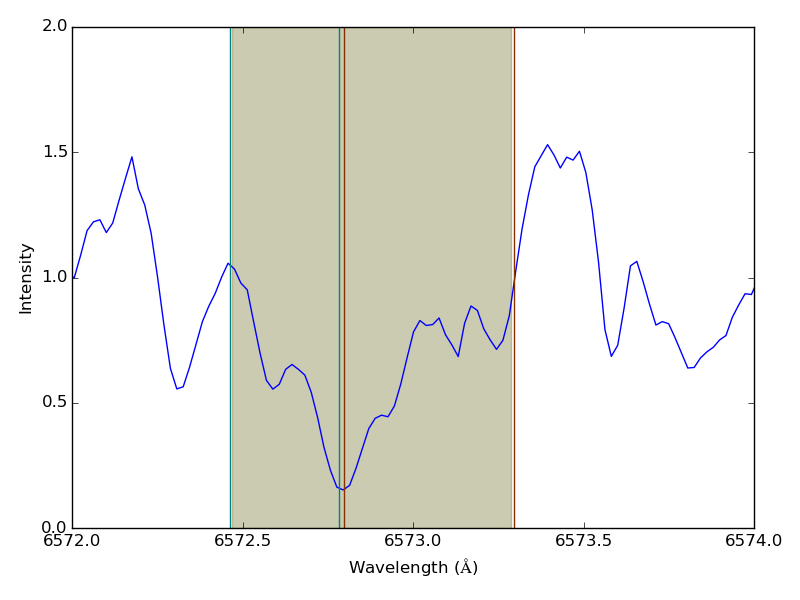
\includegraphics[scale=0.25]{Figures/tispec.png} \\
\end{center}   
\caption{This shows the section of the first spectrum in the {\harps} data (at 27 May 2004 UTC 02:10:14) used for
  calculating Equivalent Widths and also Peak Ratios from the TiO absorption line from 6572.468{\AA} to
  6573.288{\AA}. The blue vertical lines at 6572.463{\AA} and 6572.784{\AA} and the red lines at 6572.797{\AA} and
  6573.295{\AA} delineate the regions used for calculation of a version of the Peak Ratios.}
\protect\label{fig:tispec}
\end{figure}

\begin{table}[!htbp]
\centering
\scalebox{0.75}{
\begin{tabular}{|l|l|r|c|c|c|}
\hline
From & To & No. & EW  & Index & PR \\\hline
27/05/2004 & 21/07/2004 & 6 & 0.309 $ \pm $ 0.019 & 0.032 $ \pm $ 0.002 & 1.039 $ \pm $ 0.027 \\
25/07/2005 & 22/03/2006 & 5 & 0.314 $ \pm $ 0.004 & 0.032 & 1.017 $ \pm $ 0.012 \\
14/03/2007 & 19/07/2007 & 5 & 0.310 $ \pm $ 0.006 & 0.032 $ \pm $ 0.001 & 1.030 $ \pm $ 0.036 \\
29/06/2008 & 06/04/2010 & 25 & 0.315 $ \pm $ 0.007 & 0.031 $ \pm $ 0.001 & 1.020 $ \pm $ 0.035 \\
19/02/2011 & 03/06/2011 & 12 & 0.312 $ \pm $ 0.008 & 0.032 $ \pm $ 0.001 & 1.036 $ \pm $ 0.024 \\
18/01/2013 & 10/01/2014 & 207 & 0.310 $ \pm $ 0.006 & 0.032 $ \pm $ 0.001 & 1.047 $ \pm $ 0.027 \\
19/01/2016 & 30/03/2016 & 56 & 0.319 $ \pm $ 0.015 & 0.031 $ \pm $ 0.001 & 1.005 $ \pm $ 0.028 \\\hline
\multicolumn{2}{|c|}{ALL} & 316 & 0.312 $ \pm $ 0.010 & 0.032 $ \pm $ 0.001 & 1.036 $ \pm $ 0.033 \\\hline
\end{tabular}}
\caption{Results for calculation of median and standard deviation of the equivalent widths of the TiO transition at 6572.468{\AA} to
6573.288{\AA} from \harps. The observations are separated where they are 300 or more days apart.}
\protect\label{table:titable}
\end{table}

As Table \ref{table:titable} shows, an ``index'' was also considered along the same lines as the {\ha} Index, but the
size and variations (0.032 $\pm$ 0.001) were far too small to be useful.

\begin{table}[!htbp]
\centering
\scalebox{0.75}{
\begin{tabular}{|l|l|r|r|r|r|r|}
\hline
\textbf{Treatment}&\textbf{Routine}&\textbf{Peak 1}&\textbf{Peak 2}&\textbf{Peak 3}&\textbf{Peak 4}&\textbf{Peak 5}\\\hline
Original data & \scipy & 104.4 & 71.0 & 55.5 & 57.4 & 73.5 \\
EW & \astroml & 71.0 & 68.1 & 89.0 & 104.8 & 43.5 \\
 & \gatspy & 68.1 & 71.0 & 104.5 & 105.4 & 75.0 \\\hline
Original data & \scipy & 70.9 & 49.6 & 67.9 & 89.1 & 104.1 \\
EW & \astroml & 71.0 & 51.2 & 76.3 & 49.8 & 89.1 \\
Binned & \gatspy & 70.9 & 49.6 & 67.9 & 104.2 & 89.1 \\\hline
Original data & \scipy & 94.2 & 88.6 & 105.2 & 99.5 & 42.3 \\
PR & \astroml & 88.1 & 76.0 & 105.2 & 99.9 & 121.4 \\
 & \gatspy & 88.2 & 88.6 & 105.9 & 71.2 & 94.0 \\\hline
Original data & \scipy & 74.0 & 99.3 & 71.9 & 68.9 & 92.6 \\
PR & \astroml & 76.1 & 57.9 & 88.7 & 53.3 & 95.0 \\
binned & \gatspy & 99.1 & 73.8 & 71.8 & 120.1 & 121.8 \\\hline
Full data & \scipy & 97.6 & 106.2 & 109.5 & 44.3 & 70.8 \\
EW & \astroml & 42.4 & 40.8 & 46.1 & 54.1 & 50.9 \\
 & \gatspy & 106.2 & 46.0 & 97.1 & 44.2 & 75.0 \\\hline
Full data & \scipy & 121.6 & 43.6 & 40.7 & 49.5 & 108.9 \\
EW & \astroml & 47.0 & 54.2 & 49.8 & 59.4 & 43.7 \\
Binned & \gatspy & 121.6 & 43.6 & 40.7 & 49.5 & 109.0 \\\hline
Full data & \scipy & 50.6 & 42.2 & 68.0 & 106.3 & 46.1 \\
PR & \astroml & 54.1 & 46.1 & 51.6 & 60.2 & 47.0 \\
 & \gatspy & 46.1 & 68.0 & 63.1 & 50.5 & 42.3 \\\hline
Full data & \scipy & 98.2 & 121.7 & 107.6 & 106.3 & 120.4 \\
PR & \astroml & 65.8 & 47.0 & 54.1 & 71.4 & 76.6 \\
binned & \gatspy & 121.0 & 98.5 & 107.6 & 106.4 & 44.5 \\\hline
\end{tabular}}
\caption{This table shows the 5 highest peaks from the periodograms for various treatments of the TiO peak highlighted
  in Fig. \ref{fig:tispec} for Original and Full Sets of {\harps} data. The clipping where applicable was to the extreme
values of the {\ha} Equivalent Widths and binning was to 1 day.}
\protect\label{table:tipeakall}
\end{table}

As is clear, there are no periods found acceptably close to the 82.6 days argued herein to be the rotation period of
\prox. The intensity of the TiO line is clearly not great enough for any clear-cut result to be found.
